\setchapterpreamble[u]{\margintoc}
\chapter{Technical details}
\labch{practical}

Bringing all previous theoretical concepts into a working model is not straightforward if approached from scratch but, since the late 2000s and early 2010s, there have been notable advancements in programming libraries which take care of the hard work of calculating gradients and optimizing weights, leaving to the data scientist just the task of designing an appropriate model.

This chapter is dedicated to illustrating the reader on the different possibilities that exist for designing and implementing autoencoder networks. Detailed examples on how to code simple autoencoders are provided.

\section{Design}

Designing an autoencoder for a certain task can be challenging, since the objective is to find a more useful representation of the data but we cannot know the size of the optimal representation beforehand, thus difficulting decisions about the number of layers and the size of each one.

\subsection{Type of layers}

Different layers are available in every deep learning framework and can be used according to the structure of the provided data and the kind of operations the practitioner wants to apply to it.

\begin{itemize}
    \item \textbf{Unstructured variables}
    \item \textbf{Images}: the recent surge in deep learning applications is in great part due to the potential of convolutional operations for image processing. 
    \item \textbf{Sound, time series and sequential data}
\end{itemize}

\subsection{Model depth}

\subsection{Encoding layer}

\subsection{Output layer}


\section{Implementation}

During the latest years, there has been a notable evolution in the scene of software libraries for deep learning. From the existence of a wide variety of them with differing functionalities, ease of use and optimizations, there has been a tendency to condensate popularity in just two of them, which currently offer very similar functionalities and interfaces: Tensorflow and Pytorch.

\begin{figure*}[htbp]
    \centering  
    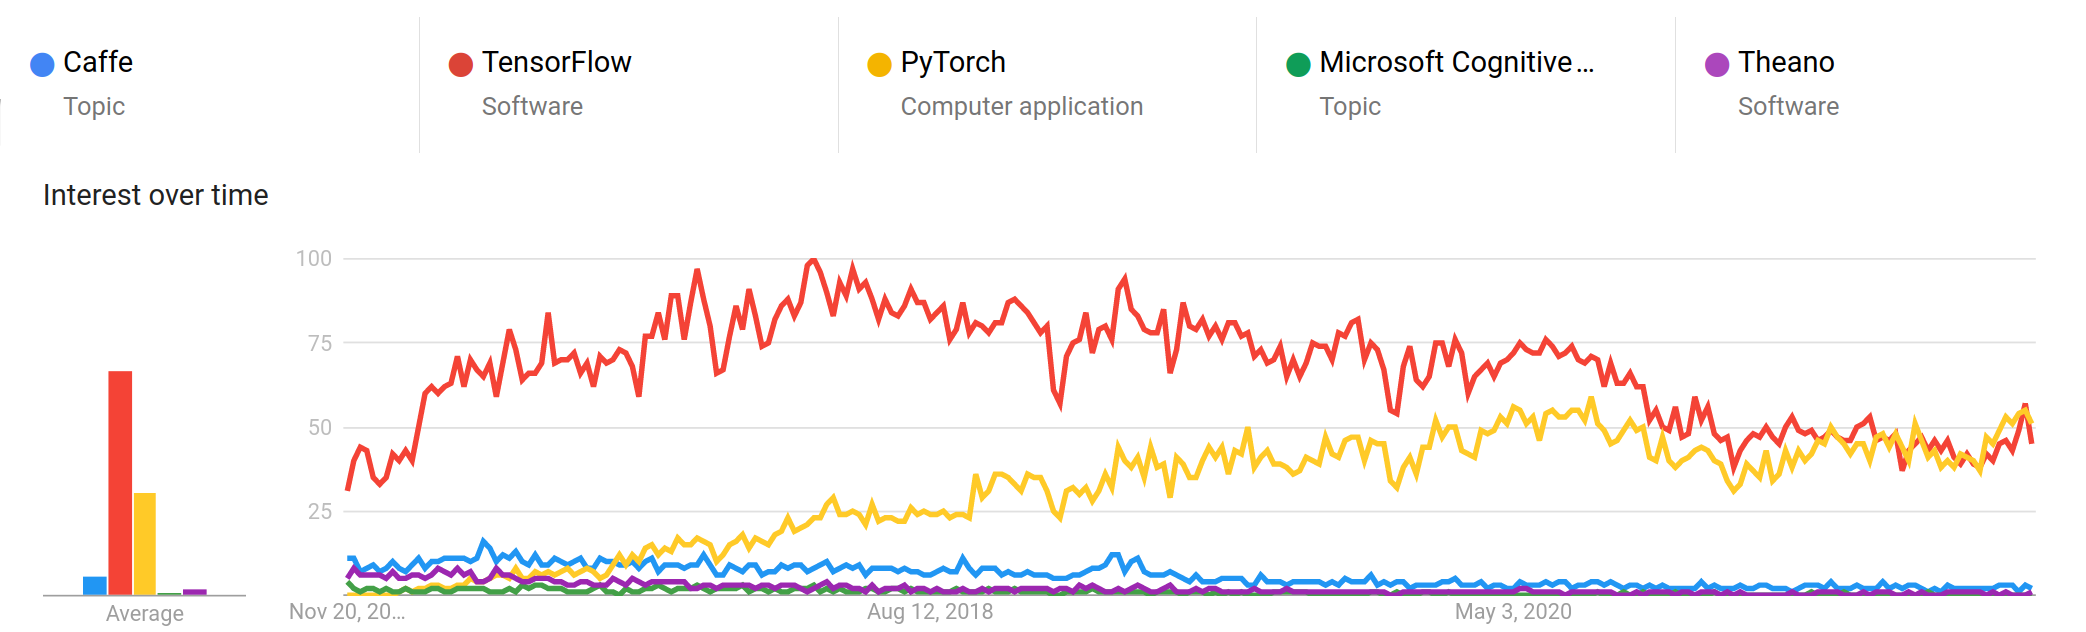
\includegraphics[width=\linewidth]{library_trends.png}
    \caption{Trends for web searches for five of the most popular deep learning frameworks, over the last 5 years.}
    \label{fig:trends}
\end{figure*}

\subsection{About Tensorflow}

- whodunnit
- main features
- small AE example

\subsubsection{Sample implementation}

Consider an essential autoencoder model where both the encoder and the decoder are composed of just one fully connected layer. 

\begin{lstlisting}[language=Python]
import tensorflow as tf

enc_dim = 10
encoder = tf.keras.Sequential([
    tf.keras.layers.Dense(enc_dim, activation="relu", 
        input_shape=(x_train.shape[1], ))
])
decoder = tf.keras.Sequential([
    tf.keras.layers.Dense(x_train.shape[1], 
        activation="sigmoid", input_shape=(enc_dim,))
])

autoencoder = tf.keras.Sequential([encoder, decoder])
autoencoder.compile(loss="binary_crossentropy", 
    optimizer="adam")
autoencoder.fit(x_train, x_train, epochs=10)
\end{lstlisting}

\subsection{About Pytorch}

\subsubsection{Sample implementation}

\begin{lstlisting}[language=Python]
import torch

encoder = torch.nn.Sequential(
    torch.nn.Linear(enc_dim),
    torch.nn.ReLU(True)
)
decoder = torch.nn.Sequential(
    torch.nn.Linear(x_train.shape[1]),
    torch.nn.Sigmoid()
)
\end{lstlisting}

- same

\section{Training deep models}

The training process of a deep learning model can be very resource-intensive, since it requires computing hundreds of arithmetic operations, usually across several thousands of parameters. 

\subsection{GPU parallelization}
